\section{Requirement 1: stochastic single-campaign environment}

% ============================================================
% Overview
% ============================================================
\begin{frame}{Stochastic single-campaign environment}
    \begin{itemize}
        \item One campaign, $T$ sequential first-price auctions
        \item Stochastic environment = stationary stochastic process, with a constant-across-rounds distribution $\mathcal{D}_m$ of the highest competing bid $m$ (unknown by the bidder)
        \item Per-round budget $\rho = B/T$, total budget $B$ (possibly $+\infty$ to model no-budget setting)
        \item Valuation $v$ of the bidder
        \item Two settings to be studied:
        \begin{itemize}
            \item \textbf{UCB-like} without budget
            \item \textbf{UCB-like} with budget
        \end{itemize}
    \end{itemize}
\end{frame}

% ============================================================
% Competing-bid distribution
% ============================================================
\begin{frame}{Competing-bid distribution: from uniform to Beta}
    % \begin{columns}[T]
    %     \begin{column}{0.5\textwidth}
    %         \textbf{Modeling choice.}
    %         \begin{itemize}
    %             \item $n$ competitors draw bids $X_i \sim \mathrm{Unif}(0,1)$
    %             \item Maximum $m = \max_i X_i \sim \mathrm{Beta}(n, 1)$
    %             \item Win probability $P(b \ge m) = b^n$
    %             \item $\Rightarrow$ classical stochastic bandit on $b \in [0,1]$ with unknown $n$
    %         \end{itemize}
    %     \end{column}
    %     \begin{column}{0.5\textwidth}
    %         \centering
    %         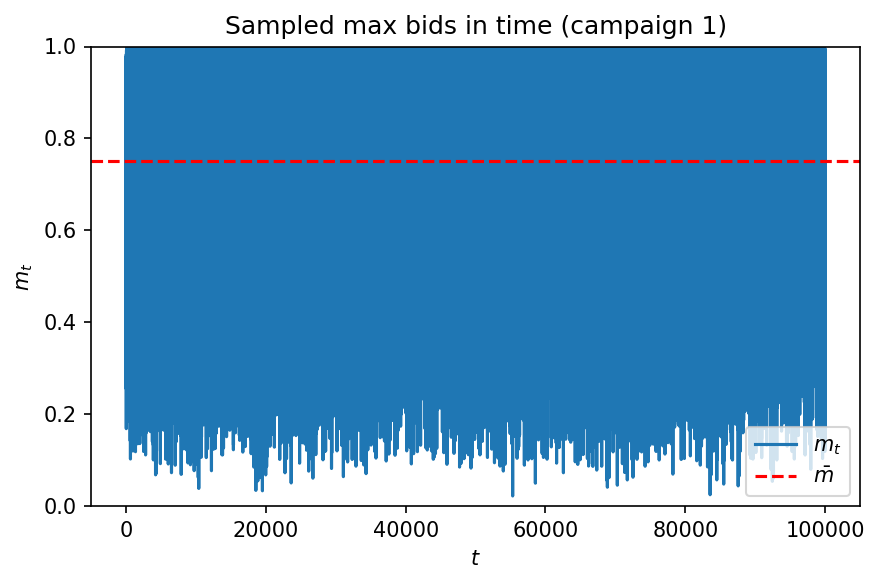
\includegraphics[width=\textwidth]{figures/req1_max_bids_ts.png}\\
    %         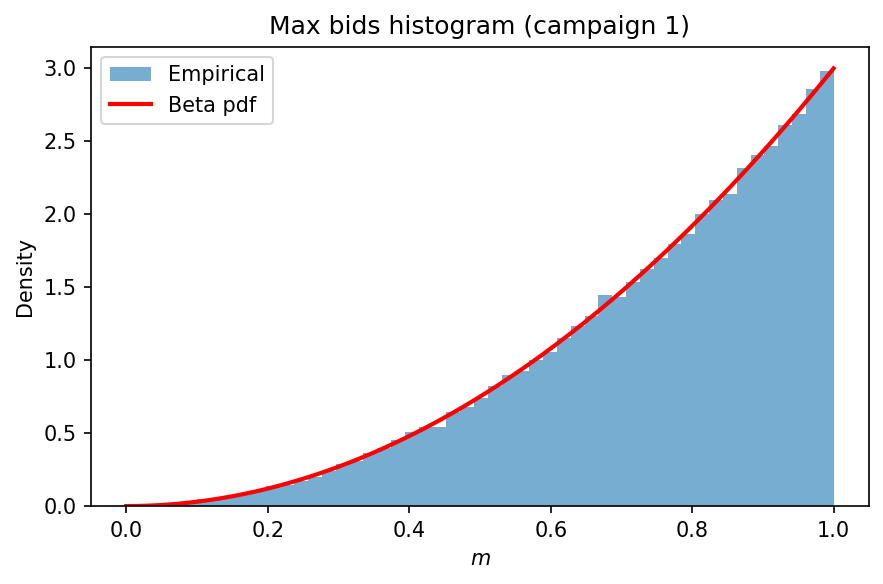
\includegraphics[width=\textwidth]{figures/req1_max_bids_hist.png}
    %     \end{column}
    % \end{columns}

    \textbf{Modeling choice:}
    \begin{columns}[T]
        \begin{column}{0.5\textwidth}
            \begin{itemize}
                \item $n$ competitors draw bids $X_i \sim \mathrm{Unif}(0,1)$
                \item Maximum $m = \max_i X_i \sim \mathrm{Beta}(n, 1)$
            \end{itemize}
        \end{column}
        \begin{column}{0.5\textwidth}
             \begin{itemize}
                \item PDF: $\mathbb{P}\left[ m = b \right] = n b^{n-1}$
                \item CDF (win probability): $\mathbb{P}\left[ m \le b \right] = b^n$
            \end{itemize}
        \end{column}
    \end{columns}
    \vspace{0.5cm}
    \centering
    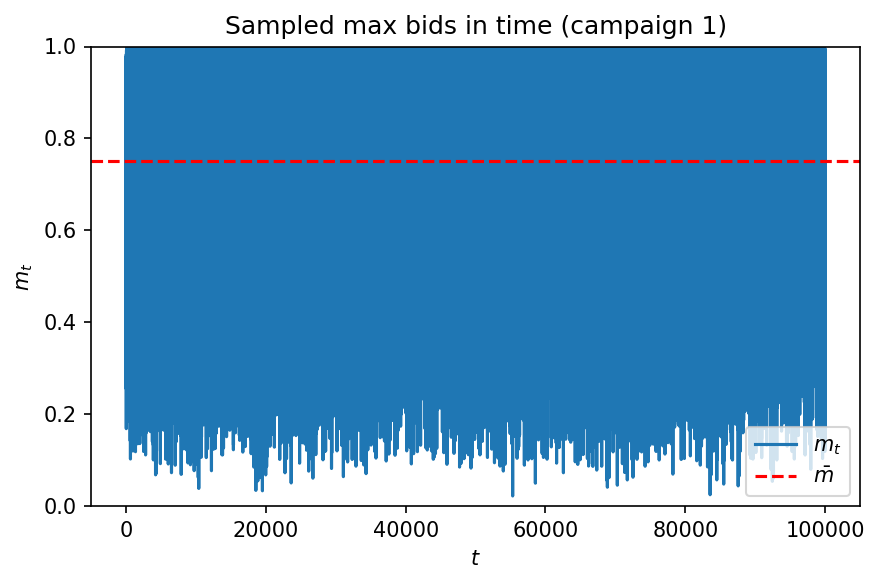
\includegraphics[width=0.4\textwidth]{figures/req1_max_bids_ts.png}
    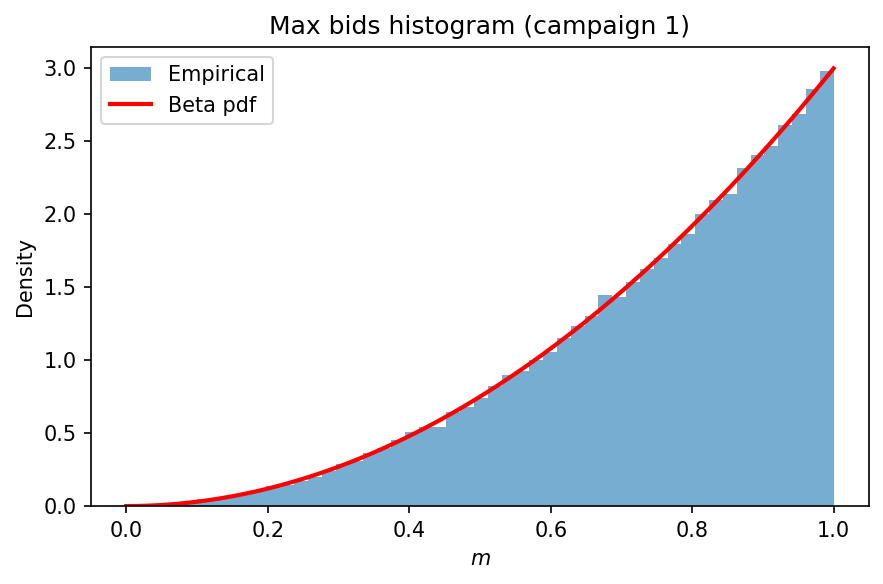
\includegraphics[width=0.4\textwidth]{figures/req1_max_bids_hist.png}
\end{frame}

% ============================================================
% Clairvoyant LP
% ============================================================
\begin{frame}{Clairvoyant}
    A clairvoyant "in expectation":
    \begin{itemize}
        \item the highest competing bids $m_t$ are stochastic and sampled from a distribution $\mathcal{D}_m$ \\
        $\implies$ we need the best behavior \emph{on average}
        \item the clairvoyant only needs to satisfy the budget constraint \emph{in expectation}, but is allowed to exceed per-round budget at any round
    \end{itemize}
    
    \begin{block}{Assumption} 
    The clairvoyant knows the underlying distribution $\mathcal{D}_m$ of the highest competing bids $m_t$, but not their actual realizations!
    \end{block}
\end{frame}

\begin{frame}{Clairvoyant - example}
    Consider the following simple setting:
    \begin{itemize}
        \item discretized bids space $\mathcal{B} = \{0.0, 0.4\}$
        \item ad valuation of the bidder $v = 0.8 \implies$ if you win, you always get a reward
        \item per-round budget $\rho = 0.2$
        \item expected highest competing bid $\mathbb{E}_{m \sim \mathcal{D}_m}\left[m\right] = 0.1$
    \end{itemize}   
\end{frame}

\begin{frame}{Clairvoyant - example}
    In this setting:
    \begin{itemize}
        \item always bidding 0.0 respects the budget constraint but never wins any auction and thus never gets any value ($f = 0.0$)
        \item always bidding 0.4 gets some value, but will likely exceed the budget constraint in expectation
    \end{itemize}

    $\implies$ a distribution over bids is needed!

    \begin{block}{} 
        There exists a single optimal bid (by existence of a deterministic policy in a stationary MDP), but we cannot use it because of the discretization of the bids space!
    \end{block}
\end{frame}

\begin{frame}{Clairvoyant - definition}
    Choose an optimal \emph{distribution} $\gamma^\star(b)$ over bids that:
    \begin{columns}[T]
        \begin{column}{0.5\textwidth}
            \centering
            maximizes the final expected reward
        \end{column}
        \begin{column}{0.5\textwidth}
            \centering
            subject to the budget constraint in expectation
        \end{column}
    \end{columns}

    \vspace{-0.2cm}
    
    \small\begin{equation*}
        \begin{aligned}
            \gamma^\star &= \arg \max_{\gamma \in \Delta_\mathcal{B}} ~~~ \bar{f}(\gamma) \qquad \qquad \qquad \qquad \qquad \qquad \qquad & \text{s.t.  } T \bar{c}(\gamma) \le B \\
            &= \arg \max_{\gamma \in \Delta_\mathcal{B}} ~~~ \bar{f}(\gamma) & \text{s.t.  } \bar{c}(\gamma) \le \rho \\    
            &= \arg \max_{\gamma \in \Delta_\mathcal{B}} ~~~ \mathbb{E}_{b \sim \gamma}\left[ \mathbb{E}_{f \sim \mathcal{D}}\left[ f(b) \right] \right] & \text{s.t.  } \mathbb{E}_{b \sim \gamma}\left[ \mathbb{E}_{c \sim \mathcal{D}}\left[ c(b) \right] \right] \le \rho \\
            &= \arg \max_{\gamma \in \Delta_\mathcal{B}} ~~~ \mathbb{E}_{b \sim \gamma}\left[ \mathbb{E}_{m \sim \mathcal{D}_m}\left[(v - b)\, \mathds{1}\left[b \ge m \right] \right] \right] & \text{s.t.  } \mathbb{E}_{b \sim \gamma}\left[ \mathbb{E}_{m \sim \mathcal{D}_m}\left[ b\, \mathds{1}\left[b \ge m \right] \right] \right] \le \rho \\    
            &= \arg \max_{\gamma \in \Delta_\mathcal{B}} ~~~ \mathbb{E}_{b \sim \gamma}\left[(v - b)\, \mathbb{E}_{m \sim \mathcal{D}_m}\left[\mathds{1}\left[ b \ge m \right] \right] \right] & \text{s.t.  } \mathbb{E}_{b \sim \gamma}\left[b\, \mathbb{E}_{m \sim \mathcal{D}_m}\left[ \mathds{1}\left[b \ge m \right] \right] \right] \le \rho \\    
            &= \arg \max_{\gamma \in \Delta_\mathcal{B}} ~~~ \mathbb{E}_{b \sim \gamma}\left[(v - b)\, \mathbb{P}_{m \sim \mathcal{D}_m}\left[b \ge m \right] \right] & \text{s.t.  } \mathbb{E}_{b \sim \gamma}\left[b\, \mathbb{P}_{m \sim \mathcal{D}_m}\left[b \ge m \right] \right] \le \rho \\    
            &= \arg \max_{\gamma \in \Delta_\mathcal{B}} ~~~ \sum_b \gamma(b)\, \underbrace{(v - b)\, \mathbb{P}_{m \sim \mathcal{D}_m} \left[b \ge m \right]}_{\bar{f}(b)} & \text{s.t.} \sum_b \gamma(b)\, \underbrace{b\, \mathbb{P}_{m \sim \mathcal{D}_m}\left[b \ge m \right]}_{\bar{c}(b)} \le \rho
        \end{aligned}
    \end{equation*}
\end{frame}

\begin{frame}{Clairvoyant - Linear Program}
    By writing the simplex constraints explicitly, we obtain the following Linear Program (LP): 
    
    \begin{equation*}
        \begin{aligned}
            \gamma^\star = \arg & \max_{\gamma \in \mathbb{R}^K} ~~~ \sum_b \gamma(b)\, \bar{f}(b) \\
            & \begin{aligned} 
                \text{s.t.} ~~~~~~ & \sum_b \gamma(b)\, \bar{c}(b) \le \rho \\
                & \sum_b \gamma(b) = 1 \\
                & 0 \le \gamma(b) \le 1\quad \forall b 
            \end{aligned}
        \end{aligned}
    \end{equation*}
\end{frame}

\begin{frame}{Clairvoyant - optimal distribution $\gamma^\star$ over bids}
    \begin{itemize}
        \item With budget, $\gamma^\star$ can concentrate on multiple bids, attempting to spend exactly the whole available budget
        \item \textbf{Note:} for $B = +\infty$ the budget constraint disappears $\implies$ we no longer care about the cost and can choose whatever deterministic bid we want, even if we overspend
    \end{itemize}
        
    \centering
    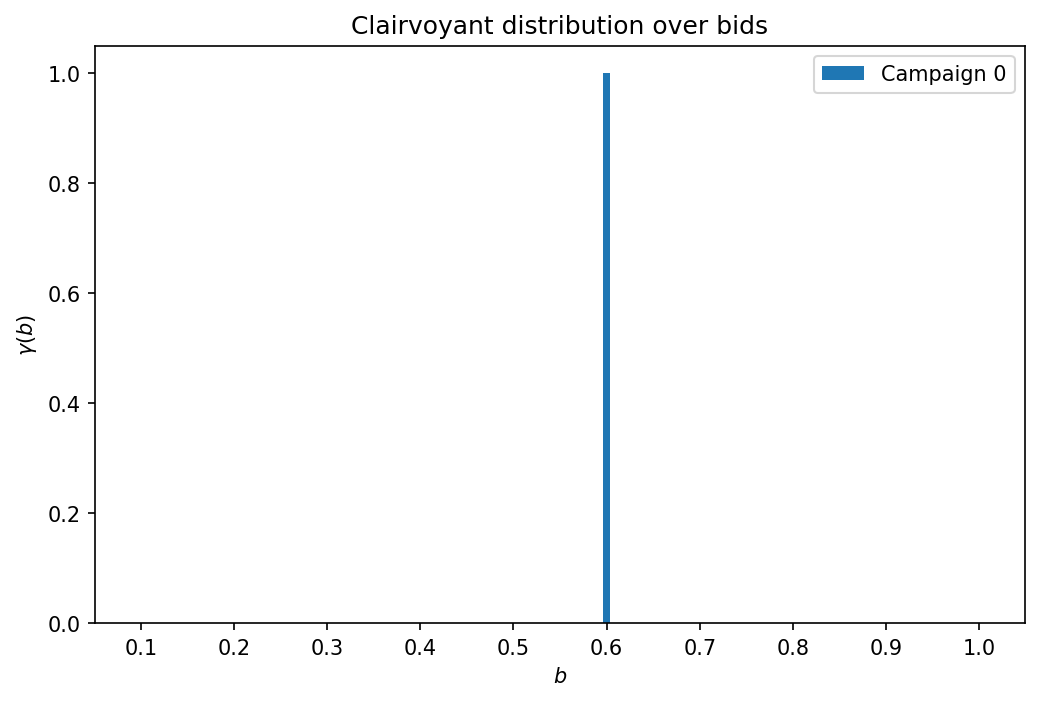
\includegraphics[width=0.35\textwidth]{figures/req1_clairvoyant_gamma_no_budget.png}
    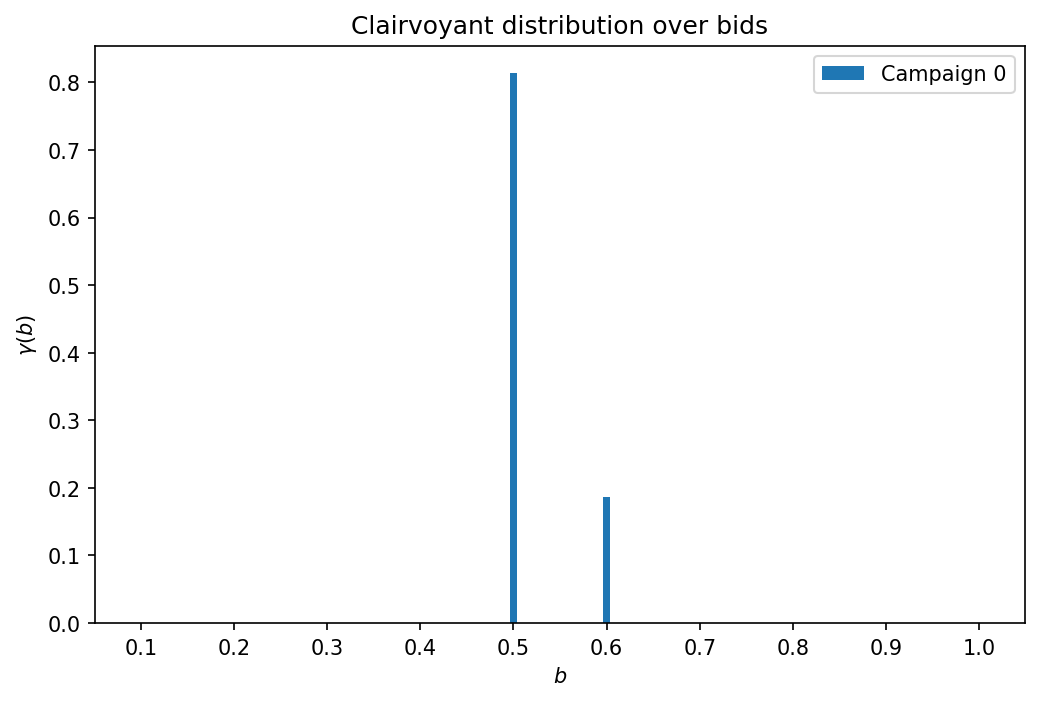
\includegraphics[width=0.35\textwidth]{figures/req1_clairvoyant_gamma_budget.png} \\
    \scriptsize
    \textbf{Left:} with no budget, the LP puts all the probability mass on the bid $b^\star$ that maximizes $\bar{f}(b) = (v - b)\,\mathbb{P}(b\ge m)$ \\ \textbf{Right:} with budget, it splits the probability mass on two adjacent bids
\end{frame}

% ============================================================
% UCB-like bidder
% ============================================================
\begin{frame}{UCB-like bidder: algorithm}
    \begin{itemize}
        \item Treat each bid $b \in \{0, 0.1, \dots, 1.0\}$ as an arm
        \item Keep track of empirical means $\hat{f}(b)$, $\hat{c}(b)$ from bandit feedback
        \item Compute the current confidence radius: \[r(b) = v \cdot \sqrt{\frac{2 \log t}{N(b)}}\]
        \item Use it to implement optimism: \[\hat{f}_{\mathrm{UCB}}(b) = \min\{\hat{f}(b)+r(b), 1\},\] \[\hat{c}_{\mathrm{LCB}}(b) = \max\{\hat{c}(b)-r(b), 0\}\]
    \end{itemize}
\end{frame}

\begin{frame}{UCB-like bidder: action selection}
    \begin{itemize}
        \item \textbf{Exploration rounds (first $K$ rounds):}  round-robin exploration of all the $K$ bids
        \item \textbf{Action selection:} we can solve the same LP as the clairvoyant, replacing the true $\bar{f}(b)$ and $\hat{c}(b)$ with the optimistic estimates
        \begin{equation*}
            \begin{aligned}
                \gamma^\star = \arg & \max_{\gamma \in \mathbb{R}^K} ~~~ \sum_b \gamma(b)\, \hat{f}_{\mathrm{UCB}} \\
                & \begin{aligned} 
                    \text{s.t.} ~~~~~~ & \sum_b \gamma(b)\, \hat{c}_{\mathrm{LCB}} \le \rho, \\
                    & \sum_b \gamma(b) = 1 \\
                    & 0 \le \gamma(b) \le 1\quad \forall b 
                \end{aligned}
            \end{aligned}
        \end{equation*}
        and then sample a bid from the resulting optimal distribution $\gamma^\star$
    \end{itemize}
\end{frame}

% ============================================================
% No-budget vs Budget comparison
% ============================================================

\begin{frame}{No-budget: empirical behavior}
    \begin{columns}[T]
        \begin{column}{0.5\textwidth}
            \centering
            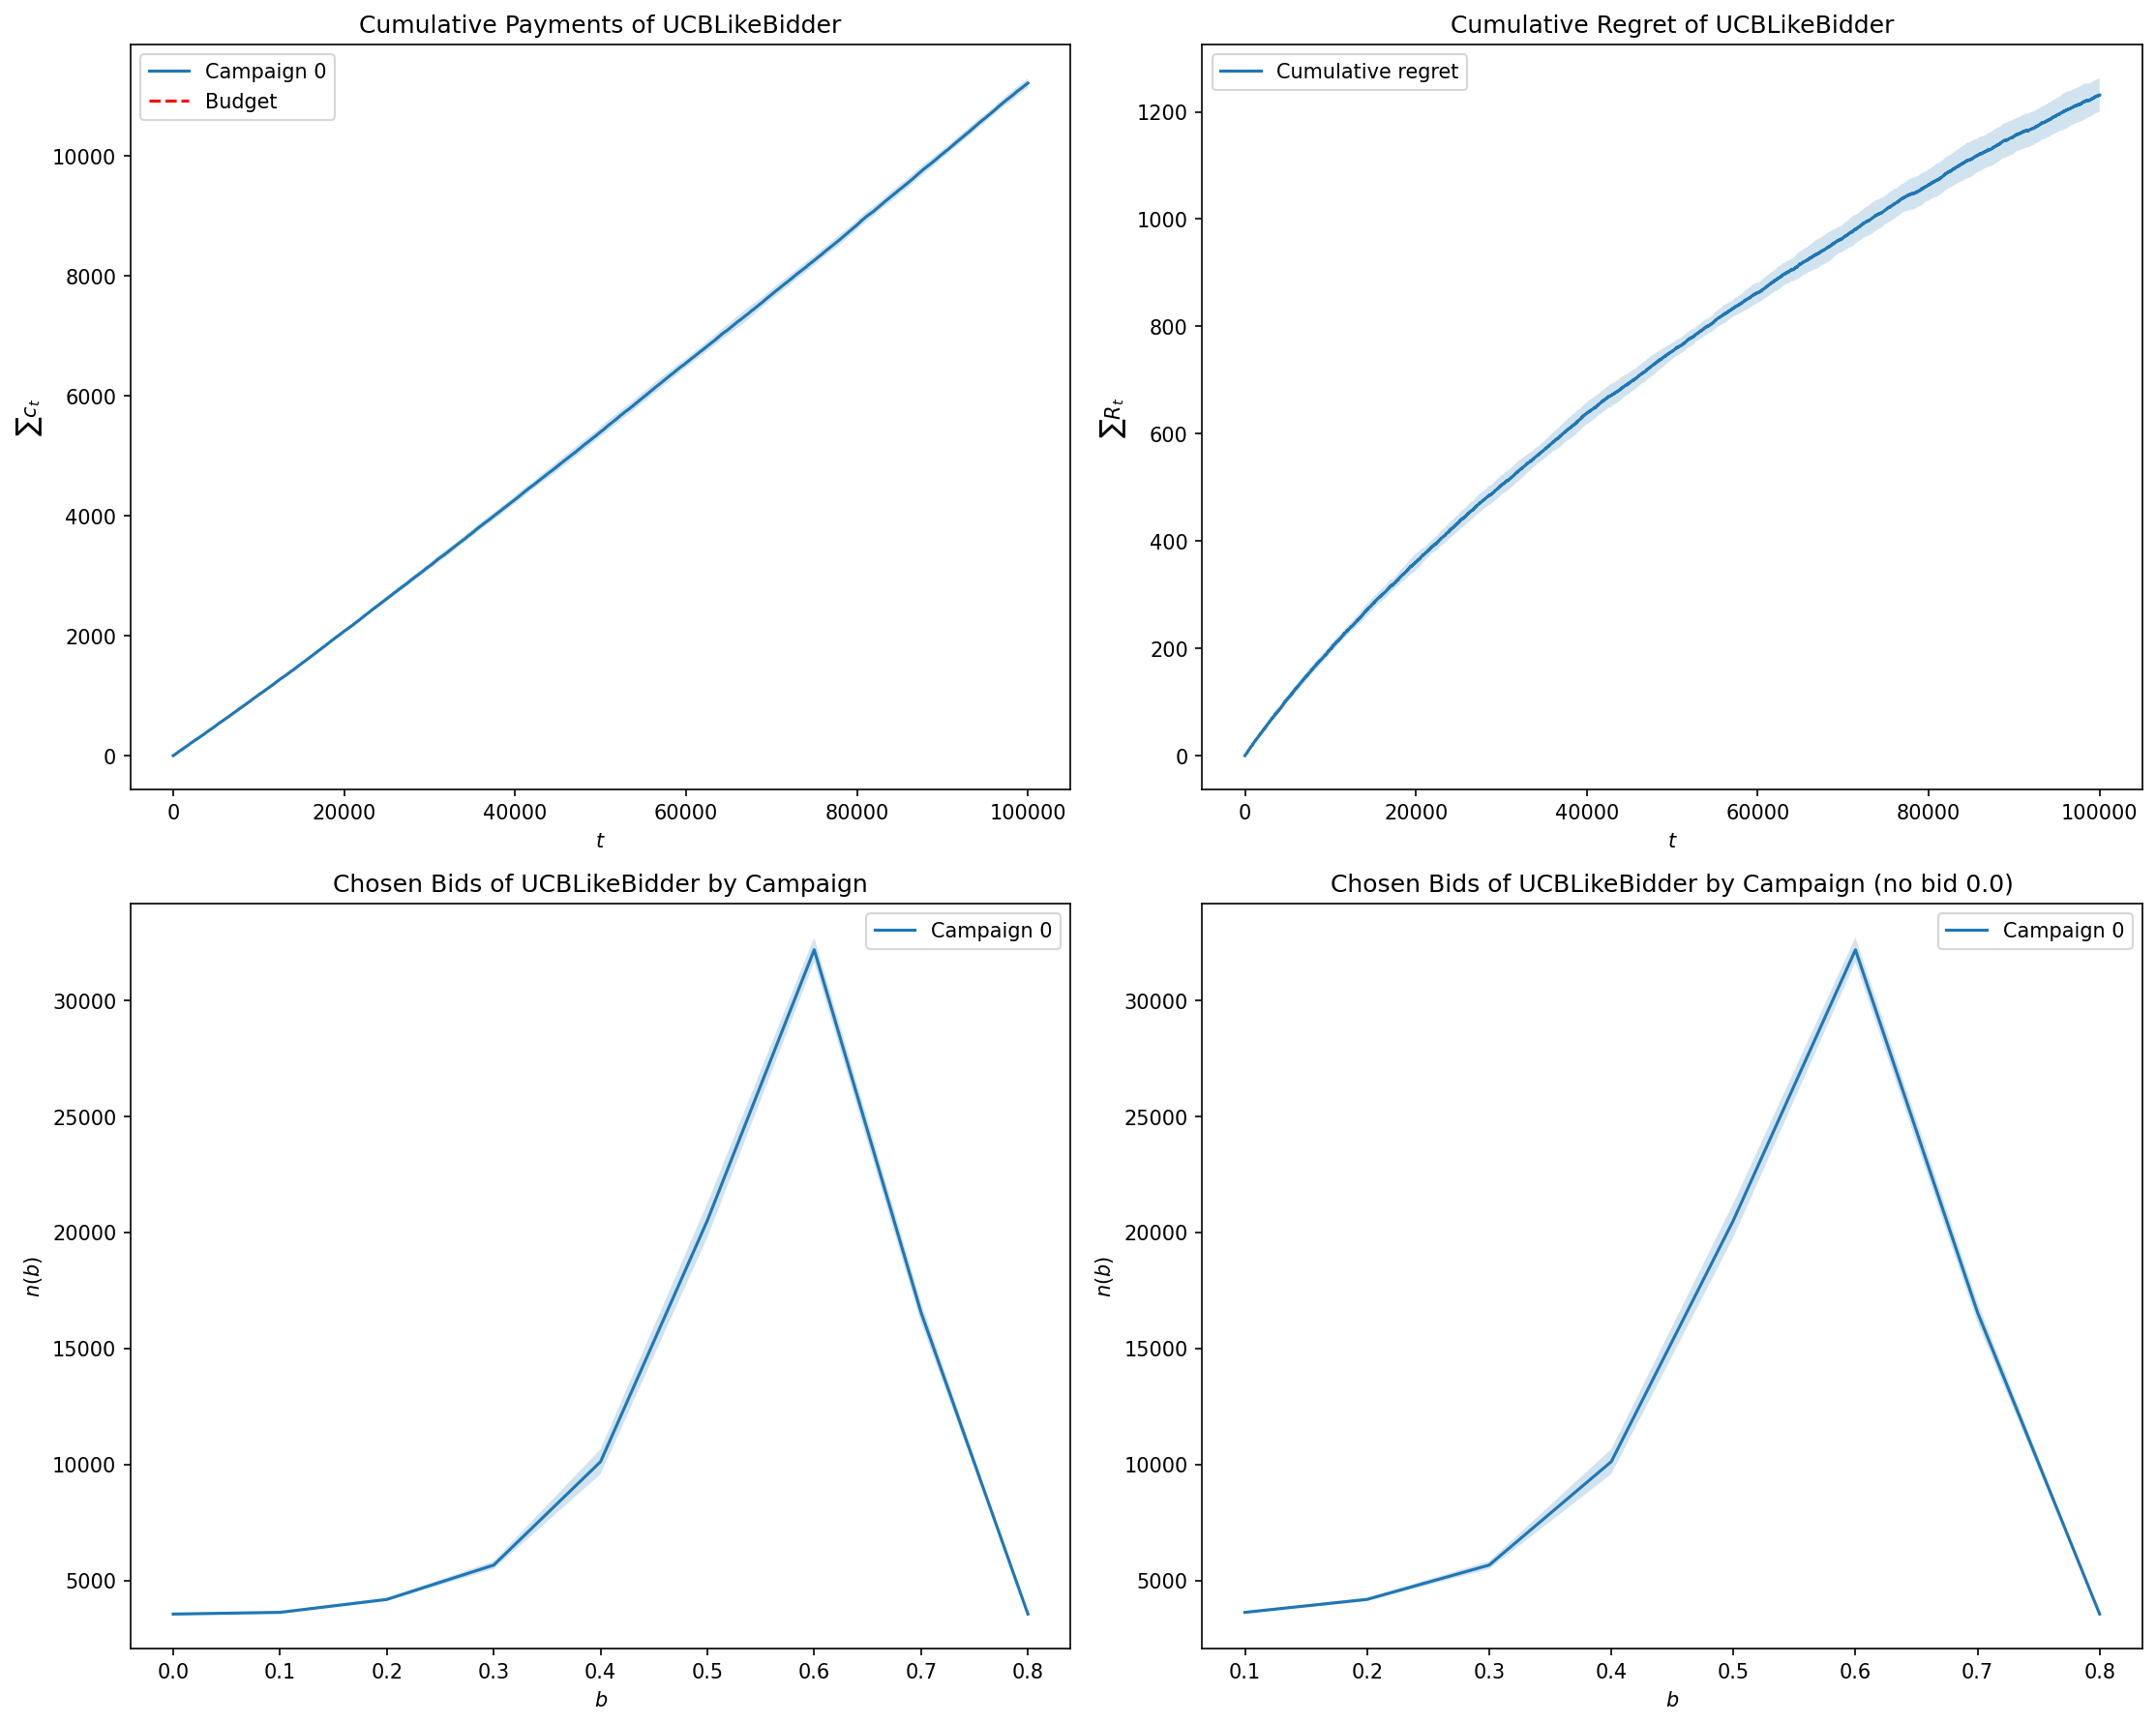
\includegraphics[width=0.95\textwidth]{figures/req1_no_budget_experiment_results.png}
            \scriptsize
            \textbf{$\rho = \infty$:} bid mass concentrates on the single arm maximizing $f_{\mathrm{UCB}}$ (matches the no-budget clairvoyant).
        \end{column}
        \begin{column}{0.5\textwidth}
             \begin{itemize}
                \item It takes $100000$ (!) rounds for the UCB-like bidder to start exhibiting sublinear regret
                \item This is because the confidence radius decay slowly for an action space of $|\mathcal{B}| = 10$ bids $\implies$ a confidence radius that decays faster should be studied 
                \item Still, the played bids are concentrating around the bid played by the no-budget clairvoyant
            \end{itemize}
        \end{column}
    \end{columns}
\end{frame}

\begin{frame}{Budget: empirical behavior}
    \begin{columns}[T]
        \begin{column}{0.5\textwidth}
            \centering
            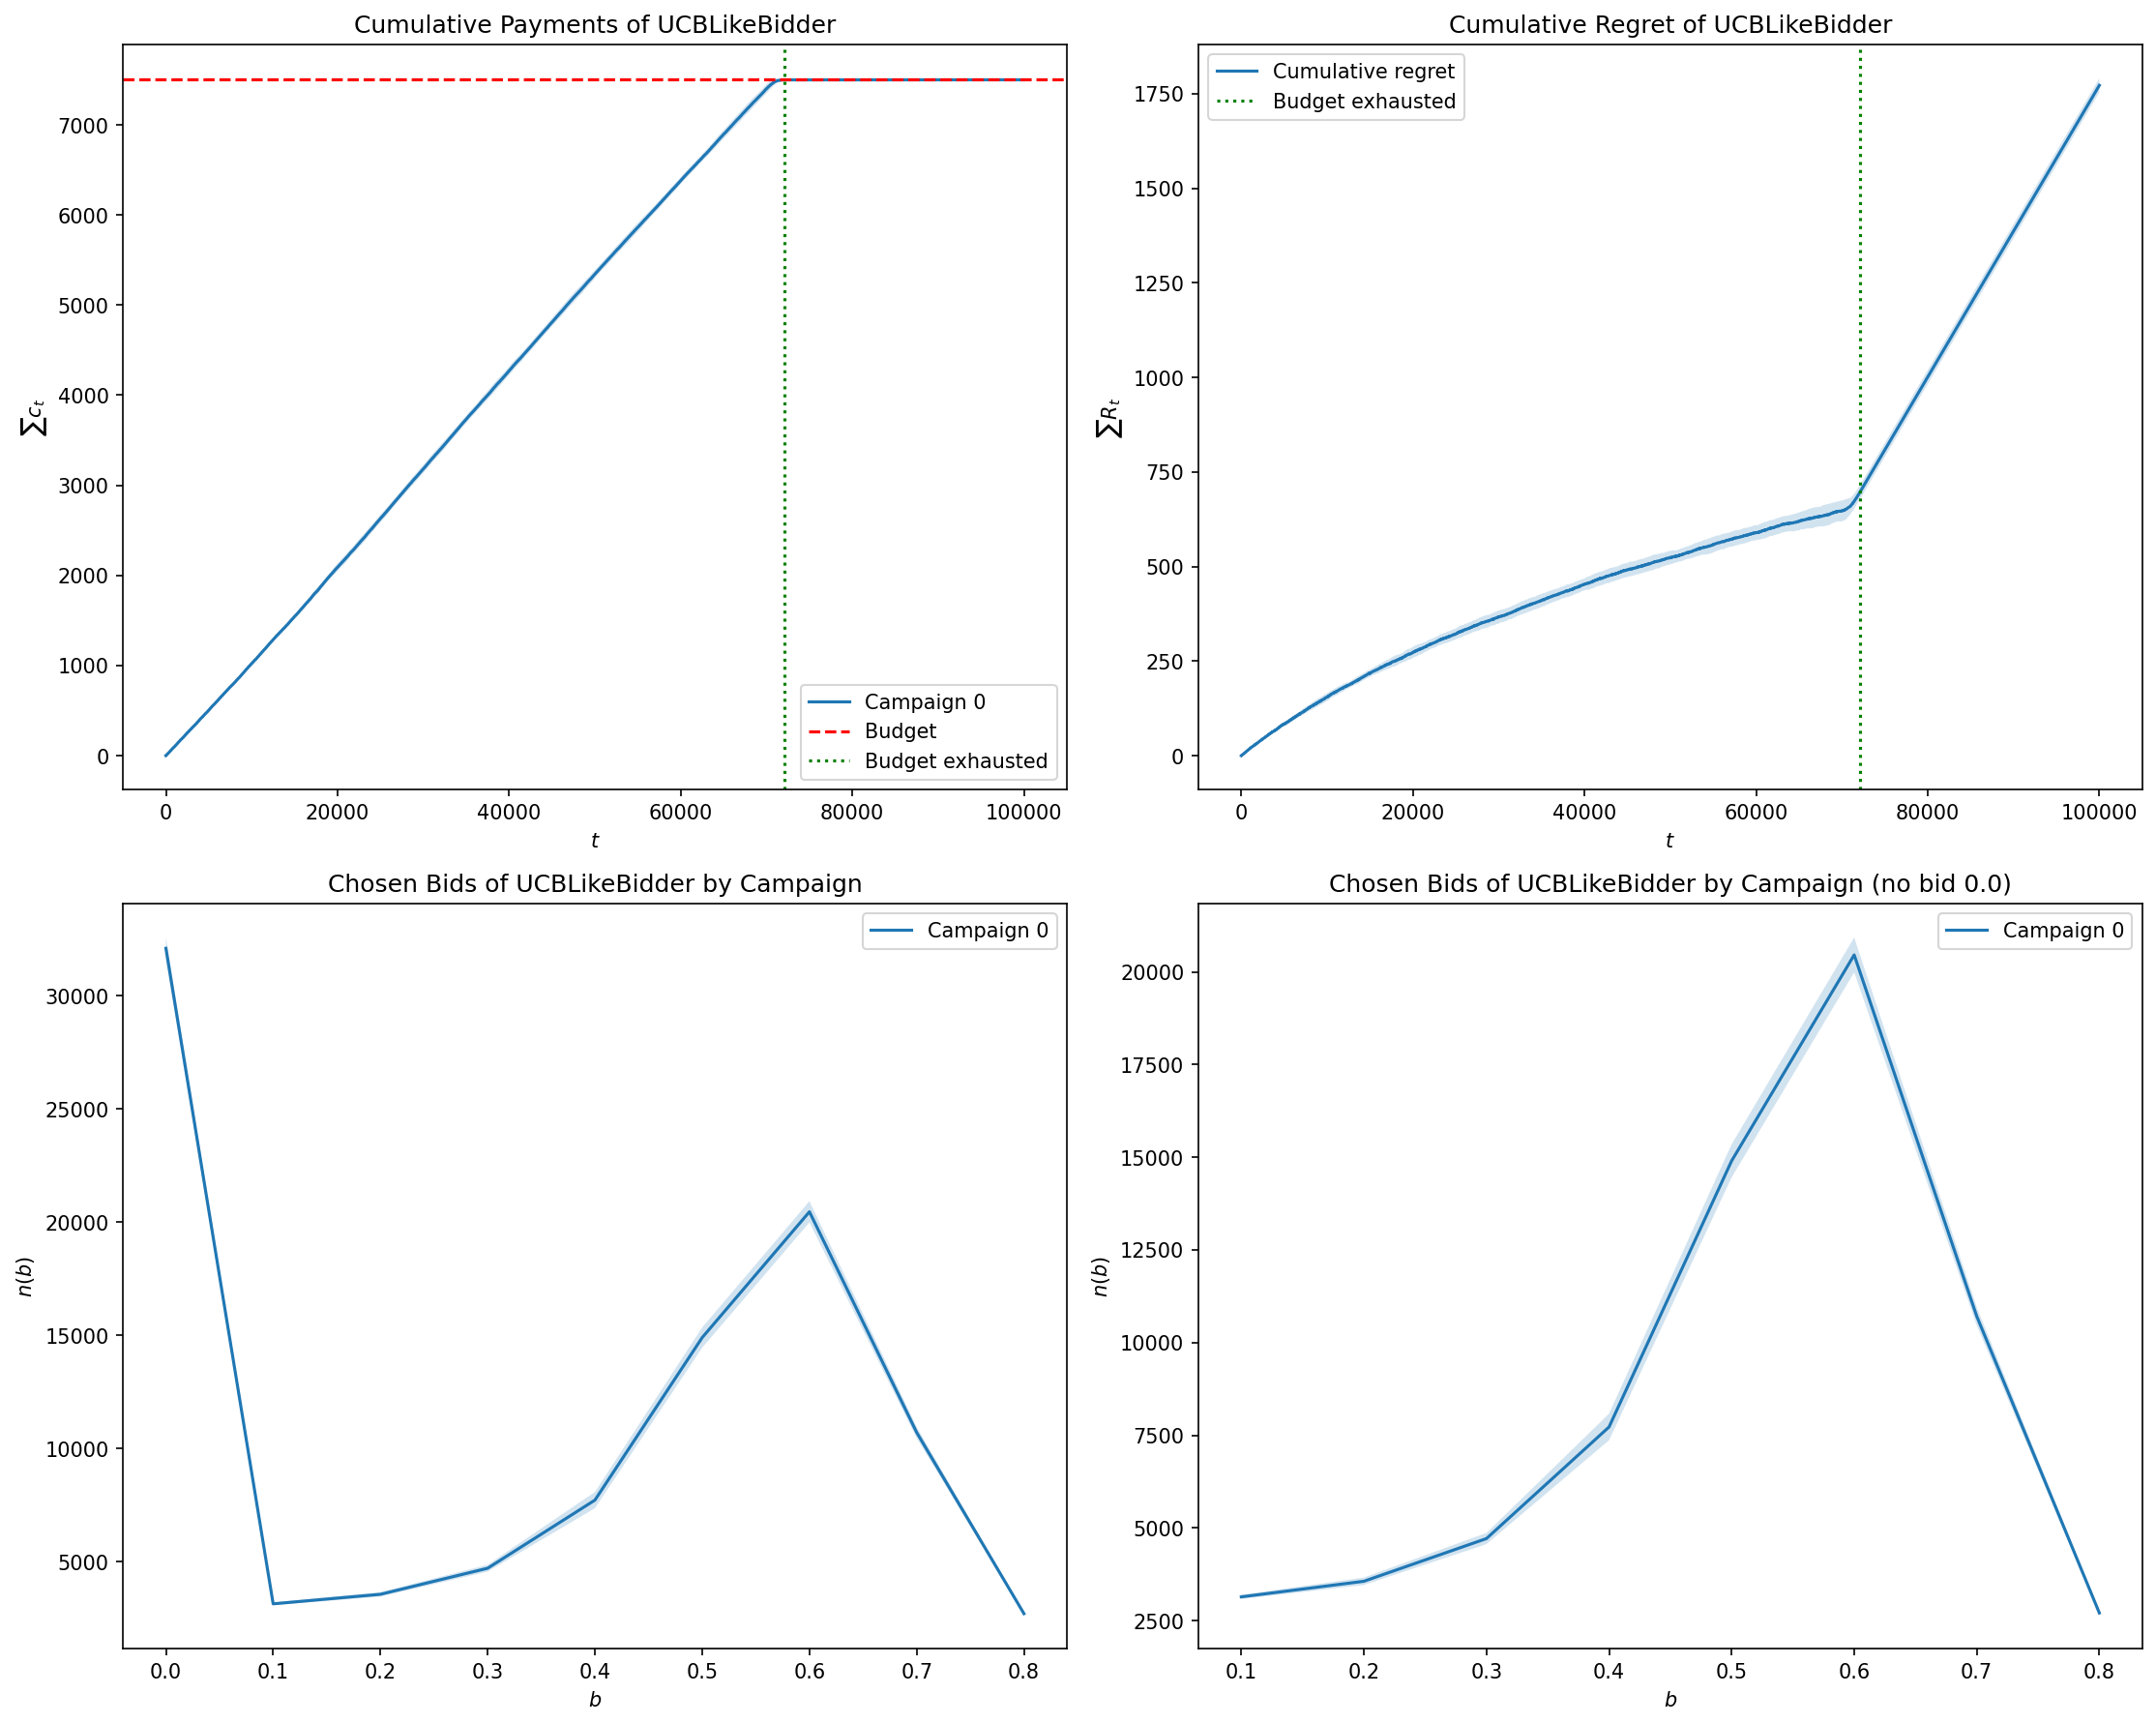
\includegraphics[width=0.95\textwidth]{figures/req1_budget_constrained_experiment_results.png}
            \scriptsize
            \textbf{$\rho < \infty$:} there are a lot of no-bid actions, because the budget gets depleted. Also, other bids are more spread out
        \end{column}
        \begin{column}{0.5\textwidth}
             \begin{itemize}
                \item Again, sublinear regret after a lot of rounds
                \item The peak in the played action is also once again concentrating around the bids played by the no-budget clairvoyant
            \end{itemize}
        \end{column}
    \end{columns}
\end{frame}

\begin{frame}{No-budget vs budget: regret comparison}
    \centering
    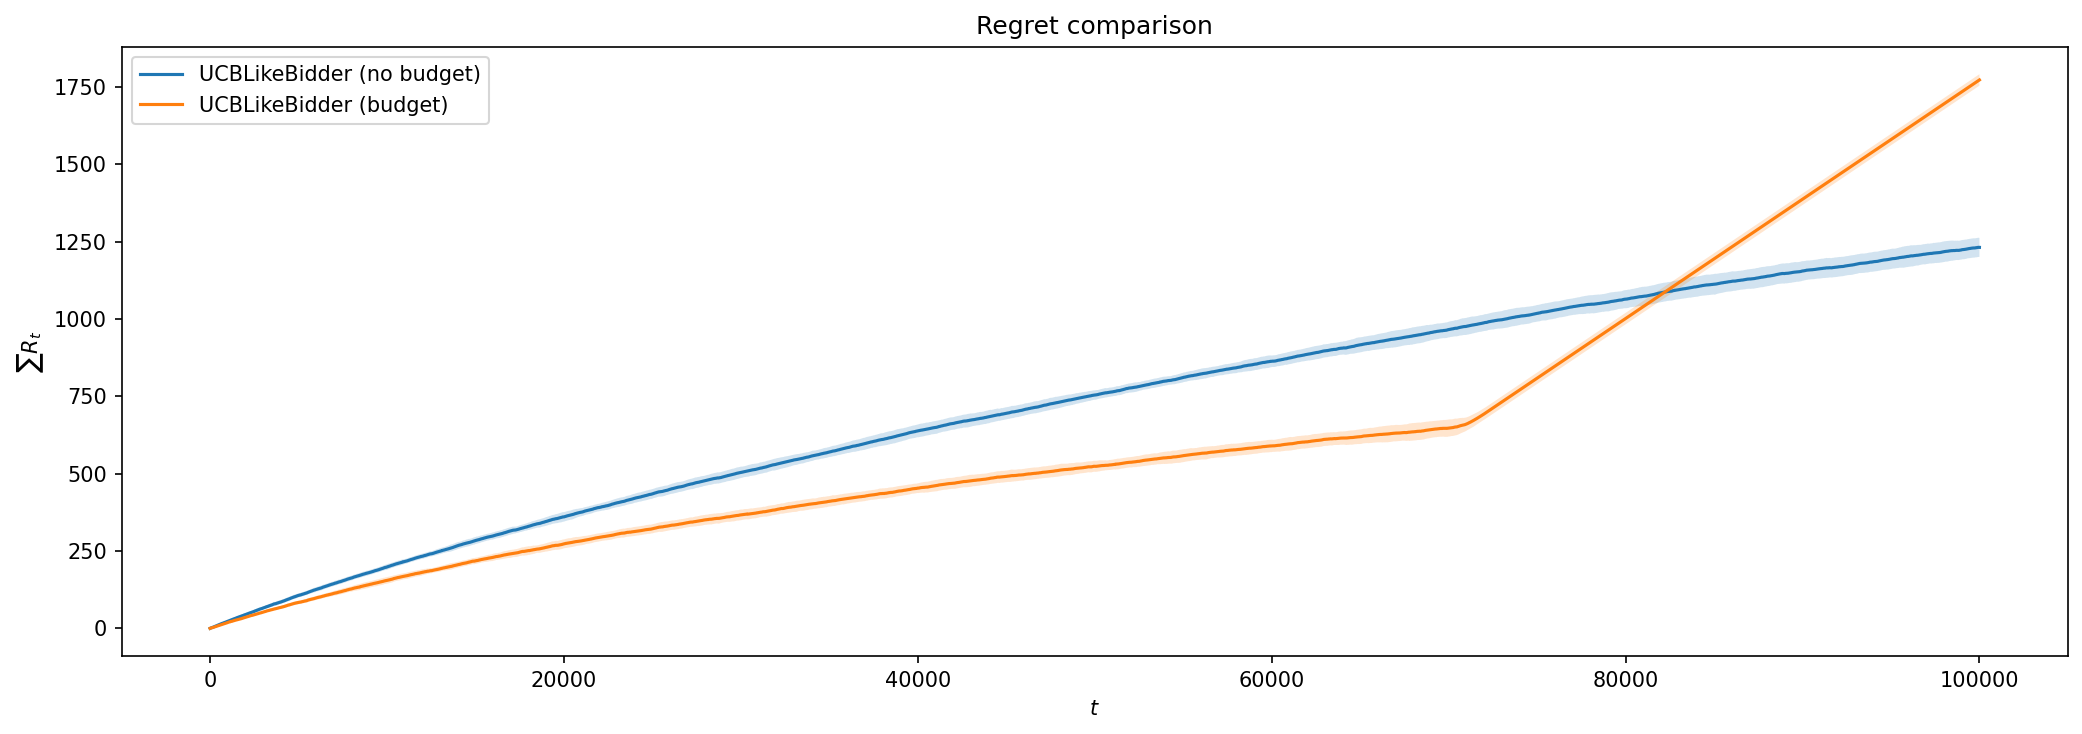
\includegraphics[width=0.9\textwidth]{figures/req1_regret_compare.png}\\
    \scriptsize
    Sublinear regret in both regimes. \textcolor{orange}{With budget}, regret is initially lower because the clairvoyant utility itself is restricted by the budget constraint; however, it eventually skyrockets when the budget is depleted, while the \textcolor{blue}{no-budget} regret keeps growing with a sublinear trend.
\end{frame}

\begin{frame}{Budget pacing}
    \centering
    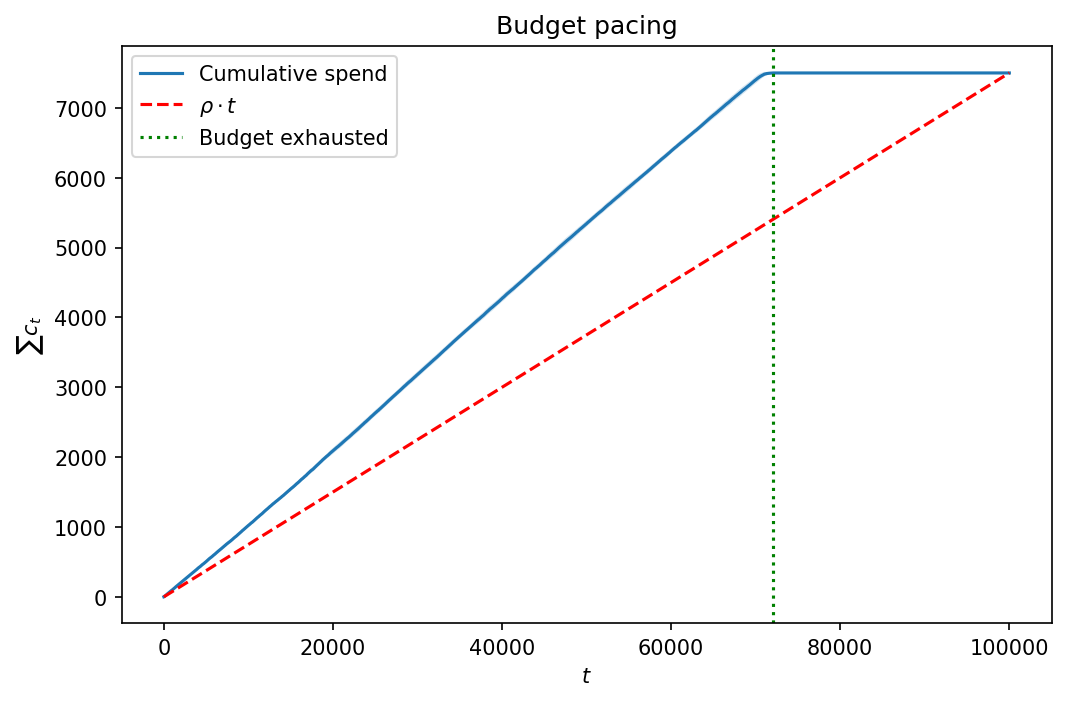
\includegraphics[width=0.37\textwidth]{figures/req1_budget_pacing.png}\hfill
    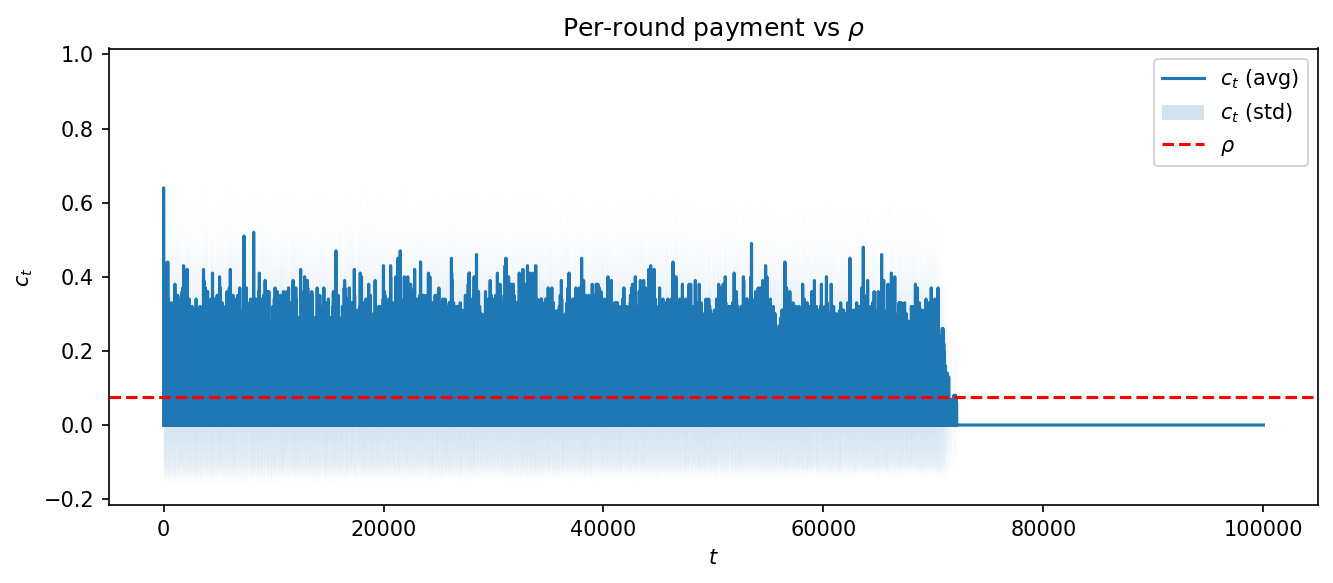
\includegraphics[width=0.57\textwidth]{figures/req1_per_round_payment_vs_rho.png}\\
    \scriptsize
    In the budget-constrained setting, we observe the bidder overspending (\textbf{left plot)}) with respect to the per-round budget $\rho$: this is likely because of exploration, as it seems to be possible to spend much more than $\rho$, while it is not possible to spend that much less (\textbf{right plot)}). 
\end{frame}
